\documentclass{standalone}
\usepackage{sheets}
\usepackage{textcomp}

\newcommand*\cellEntryB[3]{\selecCell{#1}{#2}\celtxt[l,color=red]{#1}{#2}{#3}
}


\begin{document}

\begin{tikzpicture}
\tableur[2]{A,B,C,D}
\celtxt[r]{A}{1}{1}
\celtxt[r]{B}{1}{2}
\celtxt[r]{A}{2}{10}
\cellEntry{C}{1}{=\$A1}
\end{tikzpicture} 

$\rightarrow$ Paste \texttt{C1} contents to \texttt{C2} and \texttt{D1}.

\begin{tikzpicture}
\tableur[2]{A,B,C,D}
\celtxt[r]{A}{1}{1}
\celtxt[r]{B}{1}{2}
\celtxt[r]{A}{2}{10}

\celtxt[r]{C}{1}{1}
\celtxt[r]{D}{1}{1}
\celtxt[r]{C}{2}{10}
\end{tikzpicture} 

\end{document}